\documentclass[11pt, a4paper]{article}
\setlength{\oddsidemargin}{0.5cm}
\setlength{\evensidemargin}{0.5cm}
\setlength{\topmargin}{-1.6cm}
\setlength{\leftmargin}{0.5cm}
\setlength{\rightmargin}{0.5cm}
\setlength{\textheight}{24.00cm} 
\setlength{\textwidth}{15.00cm}
\parindent 0pt
\parskip 5pt
\pagestyle{plain}

\title{Research Proposal}
\author{}
\date{}

\newcommand{\namelistlabel}[1]{\mbox{#1}\hfil}
\newenvironment{namelist}[1]{%1
\begin{list}{}
    {
        \let\makelabel\namelistlabel
        \settowidth{\labelwidth}{#1}
        \setlength{\leftmargin}{1.1\labelwidth}
    }
  }{%1
\end{list}}

\usepackage{graphicx}
\graphicspath{ {../figs/} }
\usepackage{hyperref}

\begin{document}
\maketitle

\begin{namelist}{xxxxxxxxxxxx}
\item[{\bf Title:}]
	Black Box State Change Identification Through Side Channel Analysis
\item[{\bf Author:}]
	Johnathan DiMatteo
\item[{\bf Supervisor:}]
	Sebastian Fischmeister
\end{namelist}

\section*{Motivation} 
% In this section you should give some background to your
% research area. What is the problem you are tackling, and why is it
% worthwhile solving? Who has already done some work in this area,
% and what have they achieved?

%What is IoT?

The recent explosion of the Internet of Things (IoT) puts numerous embedded devices at the hands of governments, businesses, and consumers.
Their low cost has caused manufacturers to produce and sell them without sufficient security or safety features.
If action is not taken, vulnerabilities in IoT devices can lead to harm both economically and otherwise.
To enforce security and safety in these devices, we will identify state transitions in order to reverse engineer the protocol specifications.
This way anomalies can be identified and corrected to avoid security vulnerabilities.
Traditional Hardware-in-Loop (HIL) testing methods involve significant intrusion to the system being observed.
Our approach is to monitor the execution of the system to identify transitions without opening up the so called ``black box'', a technique known as \textit{Side Channel Analysis}. 

%One proposed method to do this is a process of reverse engineering the system, called \textit{Model Learning}.
%Model learning aims to construct blackbox state diagram models of software and hardware systems by providing inputs and observing outputs.
%This has been a fundamental research problem studied for decades, but two recent advancements have allowed us to propose a new method.
%First, \textit{side channel analysis} has allowed us to study a system's response without the need to open the so called ``black box''.
%By treating a device as a black box system, one can monitor the power consumption to provide a non-intrusive approach.
%Traditional modelling tools can introduce timing errors and other anomalies. 
%The downside to this approach is the complexity of the response (ie. it is now a time series signal instead of a binary output).
%But \textit{state learning} has opened new data driven approaches for dealing with time series modeling, allowing us to cluster signals to states.
%Useful in many areas;
%one possible application could be during Hardware in the Loop (HIL) testing to identify unwanted or undocumented functionality.
%A well trained model can identify flaws in the design of IoT devices to enforce security and safety.

\section*{Problem Statement} 
%Now state explicitly the hypothesis you aim to
%test. Make references to the items listed in the Reference section
%that back up your arguments for why this is a reasonable
%hypothesis to test, for example the work of Knuth~\cite{knuth}.
%Explain what you expect will be accomplished by undertaking this
%particular project.  Moreover, is it likely to have any other
%applications?

\begin{enumerate}
    \item \textbf{Change Detector}: Given a response from a black box system, determine if the state of the system has changed in order to learn the system's behaviour.
    \item \textbf{Input Generator}: Given some inputs and knowledge of previous state changes, what should be the next query to the system?
\end{enumerate}

\section*{System}

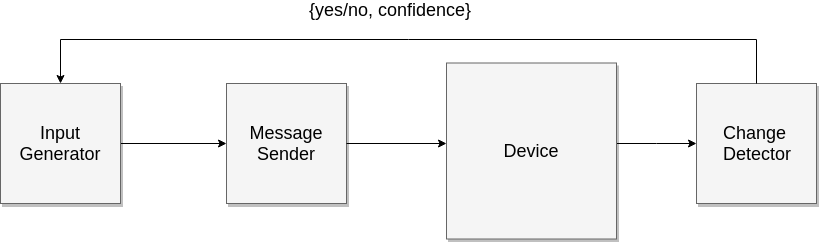
\includegraphics[scale=0.5]{change-detector.png}

\subsection*{Change Detector}
The Change Detector determines if the device has changed behaviour based on the response from the system being observed.
The response from the system is a time series signal.
The steps of the Change Detector are:
\begin{enumerate}
    \item Receive a response from the system.
    \item Determine if the state has changed.
    \item Return \{yes or no, confidence \}. 
\end{enumerate}

There are several ways to analyze time series signals:
\begin{enumerate}
    \item Distance Based
    \item Feature Based
    \item Deep Learning
\end{enumerate}

\textit{Distance Based}: using a metric to determine the similarity between two or more signals.
Common metrics include Euclidean distance and Dynamic Time Warping (DTW).
Since our response may have slight differences in timing, DTW is the best choice.

\textit{Feature Based}: using calculated features of the signal such as the mean, standard deviation, skewness, kurtosis, etc.
These features are then fed into a machine learning algorithm to determine whether or not the signal has changed.

\textit{Deep Learning}: the signals themselves are feed into multi-layered neural networks.
Similar to feature based methods except that the features are determined by the algorithms themselves.
A downside to this method is that significant data is needed for good performance.

%question: what should $\epsilon$ be? how can we tune it?\\
%question: how can we turn real valued distance into a confidence?\\

%parameters: $\epsilon$\\
%data: current state response\\
%returns: (yes/no, confidence)\\

\subsection*{Input Generator}

What message should we send to the system in order to trigger a state change?
The Input Generator should keep track of each message and the result from the Change Detector and use this information.

\begin{enumerate}
    \item Receive answer from Change Detector.
    \item Determine which message to query the system in order to try to change the state.
\end{enumerate}

There are several possible methods to determine which message to send next:
\begin{enumerate}
    \item Enumerate through all possibilities.
    \item \href{https://en.wikipedia.org/wiki/Active_learning_(machine_learning)}{Active Learning}, in particular, uncertainty sampling.
    \item \href{https://en.wikipedia.org/wiki/Genetic_algorithm}{Genetic Algorithms} to learn the best messages over time.
\end{enumerate}

\section*{Additional Modules or Functionality}
Protocol Specification: should be easy to switch from protocols. \\
Message Sender: also determined by protocol, the focus is on I2C for now.\\
Extract Protocol Method: given a list of messages that cause a state transition in the system, can a protocol be determined?

\end{document}


